\documentclass[a4paper, 11pt]{article} % Font size (can be 10pt, 11pt or 12pt)

\usepackage[protrusion=true,expansion=true]{microtype} % Better typography
\usepackage{graphicx, grffile} % Required for including pictures
\usepackage{hyperref} % Clickable cross-referencing

\usepackage{mathpazo} % Use the Palatino font
\usepackage{amsmath} % Gets \text{} working in math mode.
\usepackage[T1]{fontenc} % Required for accented characters
\linespread{2} % Change line spacing here, Palatino benefits from a slight increase by default
\usepackage[margin=1.5in]{geometry}
\usepackage{changepage}
\usepackage{collectbox}
\usepackage{float}

\makeatletter
\newcommand{\sqbox}{%
	\collectbox{%
		\@tempdima=\dimexpr\width-\totalheight\relax
		\ifdim\@tempdima<\z@
		\fbox{\hbox{\hspace{-.5\@tempdima}\BOXCONTENT\hspace{-.5\@tempdima}}}%
		\else
		\ht\collectedbox=\dimexpr\ht\collectedbox+.5\@tempdima\relax
		\dp\collectedbox=\dimexpr\dp\collectedbox+.5\@tempdima\relax
		\fbox{\BOXCONTENT}%
		\fi
	}%
}
\makeatother

\makeatletter
\renewcommand\@biblabel[1]{\textbf{#1.}} % Change the square brackets for each bibliography item 
%from '[1]' to '1.'
\renewcommand{\@listI}{\itemsep=0pt} % Reduce the space between items in the itemize and 
%enumerate environments and the bibliography
\renewcommand{\sectionautorefname}{\S}

\renewcommand{\maketitle}{
\begin{flushright}
	{\LARGE\@title}
	\vspace{50pt} \\
	{\large\@author}
	\\\@date
	\vspace{40pt}
\end{flushright}
}

\title{
	\begin{figure}
		\begin{center}
					
\includegraphics[width=8cm]{figures/logo.jpg}
		\end{center}
	\end{figure}	
	\textbf{ST3288 UROPS Report
}\\
Applying machine learning techniques to determine the occupancy of parking lots}

\author{\textsc{Rayakar Achal Ajeet, A0156139B}\\
		\texttt{\hyperlink{achal@u.nus.edu}{achal@u.nus.edu}}\\
		\textit{National University of Singapore}
}

\date{7th August, 2018}

%----------------------------------------------------------------------------------------

\begin{document}

\maketitle % Print the title section

\newpage

\tableofcontents

\newpage

\section{Summary}
    This report discusses the conclusion of the two-semester UROPS project entitled ``Parking Lot
    Classification''; namely, it details the suite of tools developed and results achieved in the effort to use
    convolutional neural networks (CNNs) to ascertain the state of a parking lot given its picture. The 
    report will briefly recount the first semester's results, and intentions before delving into how these 
    motivations developed in the second.
\newpage
\section{Recount of ST2288: ``Parking Lot Classification''}
	The motivation behind investigating the use of CNNs in this task was to determine whether it was 
	possible to reliably and inexpensively increase the resolution of information available to drivers 
	looking for parking space; in Singapore, most public parking lots provide users with the number of 
	spots left, but not \textit{where} such spots are. When parking is scarce, traversal to find free spots 
	can be a great inconvenience. Thus, an Internet-of-Things idea based on the usage of 
	already-installed CCTV cameras was proposed to be tested:
	\begin{center}
		\textbf{
			how can one use the \textit{image} of a parking lot to determine its spot-wise occupancy, and 
			then deliver this information to users, in real-time?
		}
	\end{center}
	CNNs were selected to be the classification model behind this idea's implementation since they are 
	currently state-of-the-art for many computer vision tasks.
	The  following was the proposed workflow of a system based on this idea: 
	\begin{enumerate}
		\item User requests for spot-wise occupancy status of a given parking lot through a mobile 
		application created to handle such requests in real-time.
		\item A picture of the lot is taken by a pre-existing CCTV or dedicated camera, and transmitted to 
		the associated cloud-based CNN.
		\item Each spot in the parking lot is classified by this CNN as either empty or occupied.
		\item The picture is then deleted, and the is user sent a spatially-accurate abstraction of 
		spot-wise occupancy status (possibly in the manner pictured below).
	\end{enumerate}
	\begin{figure}[H]
		\centering
		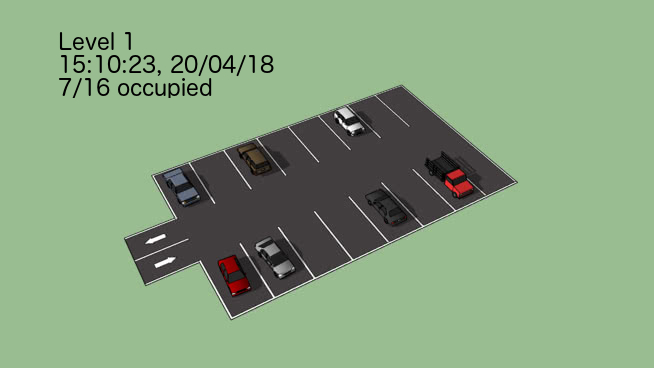
\includegraphics[width=8cm]{figures/mock-up.jpg}
		\caption{This visual could be delivered to users through the mobile application.}
	\end{figure}
	The focus of the previous semester's work was solely the third step of the above workflow: to 
	explore and determine the effectiveness of CNNs for this classification task. To this end, CNNs were 
	found to work very well. A publicly-available parking lot image dataset, \textit{PKLot}, was used to 
	train, validate, and test CNNs created\footnote{This dataset can be found at: 
	\hyperlink{https://web.inf.ufpr.br/vri/databases/parking-lot-database/}
	{web.inf.ufpr.br/vri/databases/parking-lot-database/}}. It comprises of 695,899 images of 
	parking spots taken from two parking lots over the course of about 30 days, in which there was 
	great variation of weather and illumination \cite{pklot-paper}\relax. The following are three example 
	images from this dataset:
	\vskip 5mm
	\begin{figure}[H]
		\centering
		
\includegraphics[width=1cm]{figures/pklot_example_1.jpg}
		\caption{An occupied spot from the first parking lot, in sunshine.}
	\end{figure}
	\begin{figure}[H]
		\centering
		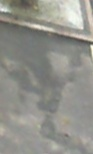
\includegraphics[width=1cm]{figures/pklot_example_2.jpg}
		\caption{An empty spot from one angle of the second parking lot, in overcast conditions.}
		\vspace{5mm}
		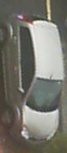
\includegraphics[width=1cm]{figures/pklot_example_3.jpg}
		\caption{An occupied spot from the second angle of the second parking lot, in rain.}
	\end{figure}
	\hspace*{-6mm}The testing accuracies of the CNNs created for each lot in this dataset were greater 
	than 99.8\%, which translates to the misclassification of about 260 spots in requesting for the 
	prediction of the state of about 175,000.The following was their architecture:
	\begin{itemize}
		\item[] An input layer which reads in 32-by-32 color images of parking spots.
		\item[] Convolutional layer 1: applies 32 5-by-5 filters, and then applies the ReLU activation 
		function.
		\item[] Pooling layer 1: performs max pooling with a 2-by-2 filter.
		\item[] Convolutional layer 2: applies 64 3-by-3 filters, and then applies the ReLU activation 
		function.
		\item[] Pooling layer 2: performs max pooling with a 2-by-2 filter.
		\item[] Fully-connected layer 1: comprises of 1,024 neurons/predictors.
		\item[] Output layer: 2 neurons, representing the output vector.
		\vspace*{-4mm}
		\begin{enumerate}
			\setlength\itemsep{-3mm}
			\item[] (0, 1) $\rightarrow$ occupied spot
			\item[] (1, 0) $\rightarrow$ empty spot
		\end{enumerate}
	\end{itemize}
   	The CNNs were implemented using \href{https://www.tensorflow.org}{TensorFlow}, an efficient and 
   	well-supported deep-learning library written for the Python programming language. Training and 
   	testing of the CNNs was done online on \href{https://www.floydhub.com}{FloydHub}. FloydHub is a 
   	Platform-as-a-Service that quite inexpensively offers a pre-configured programming environment on 
   	powerful hardware for machine learning purposes. Users run ``jobs'' through a command-line client, 
   	with data and algorithms stored on FloydHub. Training metrics and logs can also be automatically 
    generated:
    \vskip 5mm
    \begin{figure}[H]
    	\centering
    	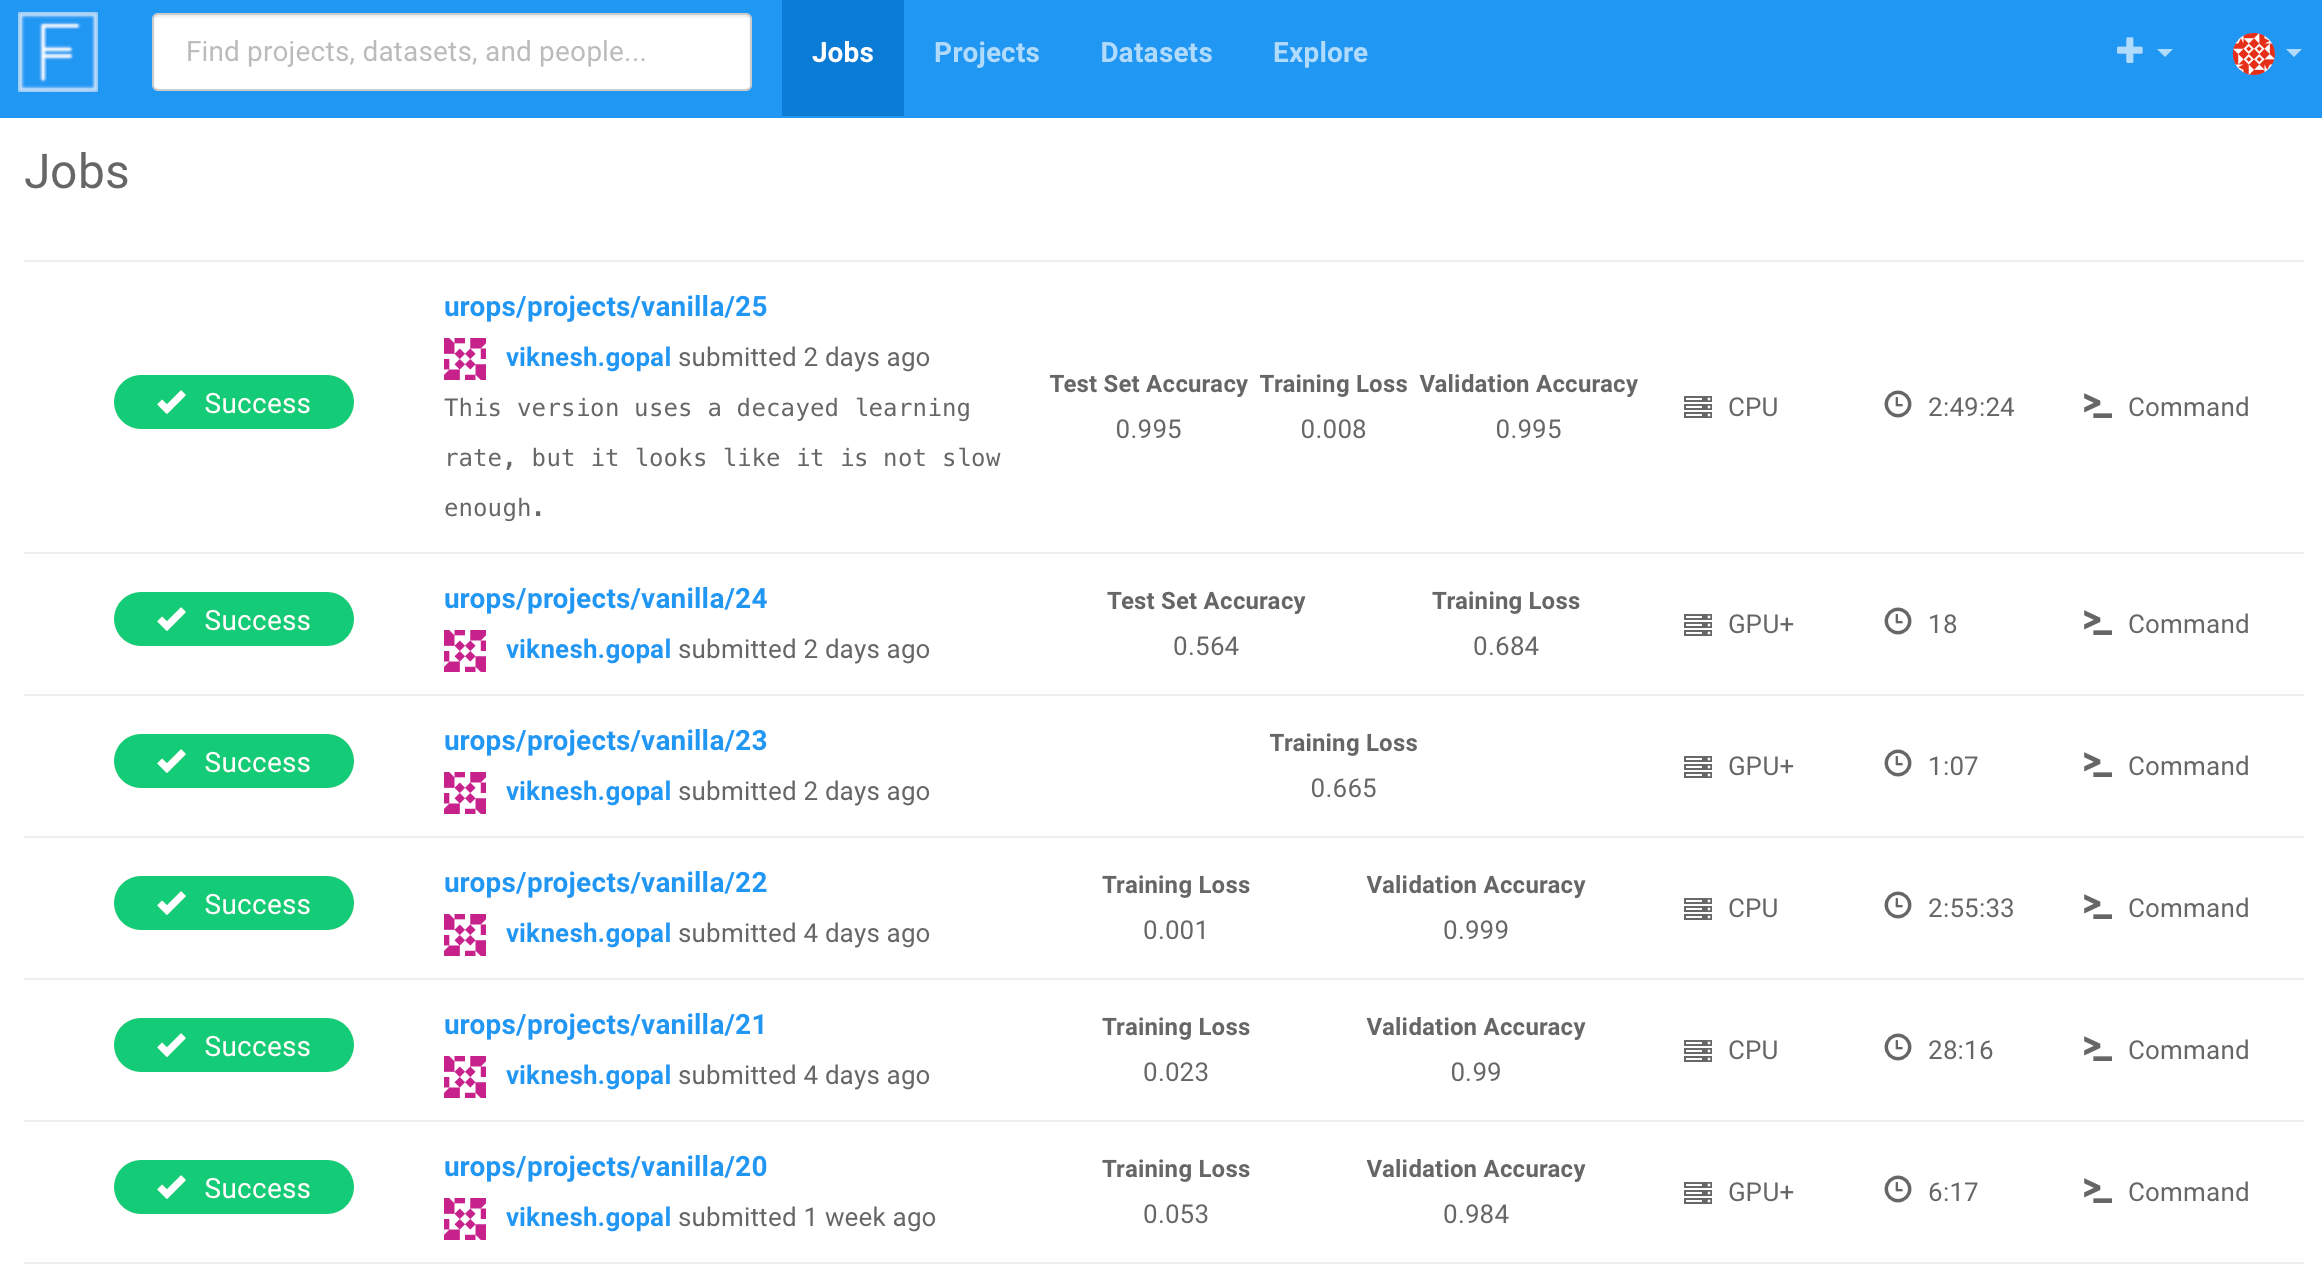
\includegraphics[width=14cm]{figures/floydhub.png}
    	\caption{Log of jobs run on FloydHub.}
    \end{figure}
	\newpage
	With the above results and tools, ST2288 was concluded. This left trialling of the practical 
	application of this idea in the local context to ST3288. The rest of this report details the unique 
	challenges involved in the creation and management of original data, the tools created in response, 
	and the deep generalizability of the resulting CNN-creation workflow to other machine learning 
	projects. The algorithms and files referred to in this report are as they are found on  
	\hyperlink{https://github.com/nurmister/urops}{github.com/nurmister/urops}.
\newpage
\section{Creation of \textit{NUSLot}}
	\textit{NUSLot} is the culmination of the data collection, processing, and labeling efforts of this 
	project; it comprises of 50,000 labeled examples of spots of the parking lot belonging to block 
	S17 at the Faculty of Science\footnote{This dataset can be found at: 
	\hyperlink{https://goo.gl/fV2NXS}{goo.gl/fV2NXS}}. The following are three example images 
	from this dataset:
	\vskip 5mm
	\begin{figure}[H]
		\centering
		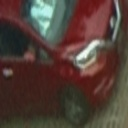
\includegraphics[width=2cm]{figures/nuslot_example_1.jpg}
		\caption{An occupied spot.}
		\vspace{5mm}
		
\includegraphics[width=2cm]{figures/nuslot_example_2.jpg}
		\caption{An empty spot.}
		\vspace{5mm}
		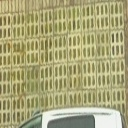
\includegraphics[width=2cm]{figures/nuslot_example_3.jpg}
		\caption{Another empty spot. Notice the occlusion caused by the roof of the vehicle occupying 
		the adjacent spot.}
	\end{figure}
	\hspace*{-6mm}More specifically, this dataset consists of 50,000 128-by-128 pixel BGR images of 
	parking spots, taken between the fourteenth of June and the 24th of July. These images were taken 
	from the following vantage:
	\vskip 5mm
	\begin{figure}[H]
		\centering
		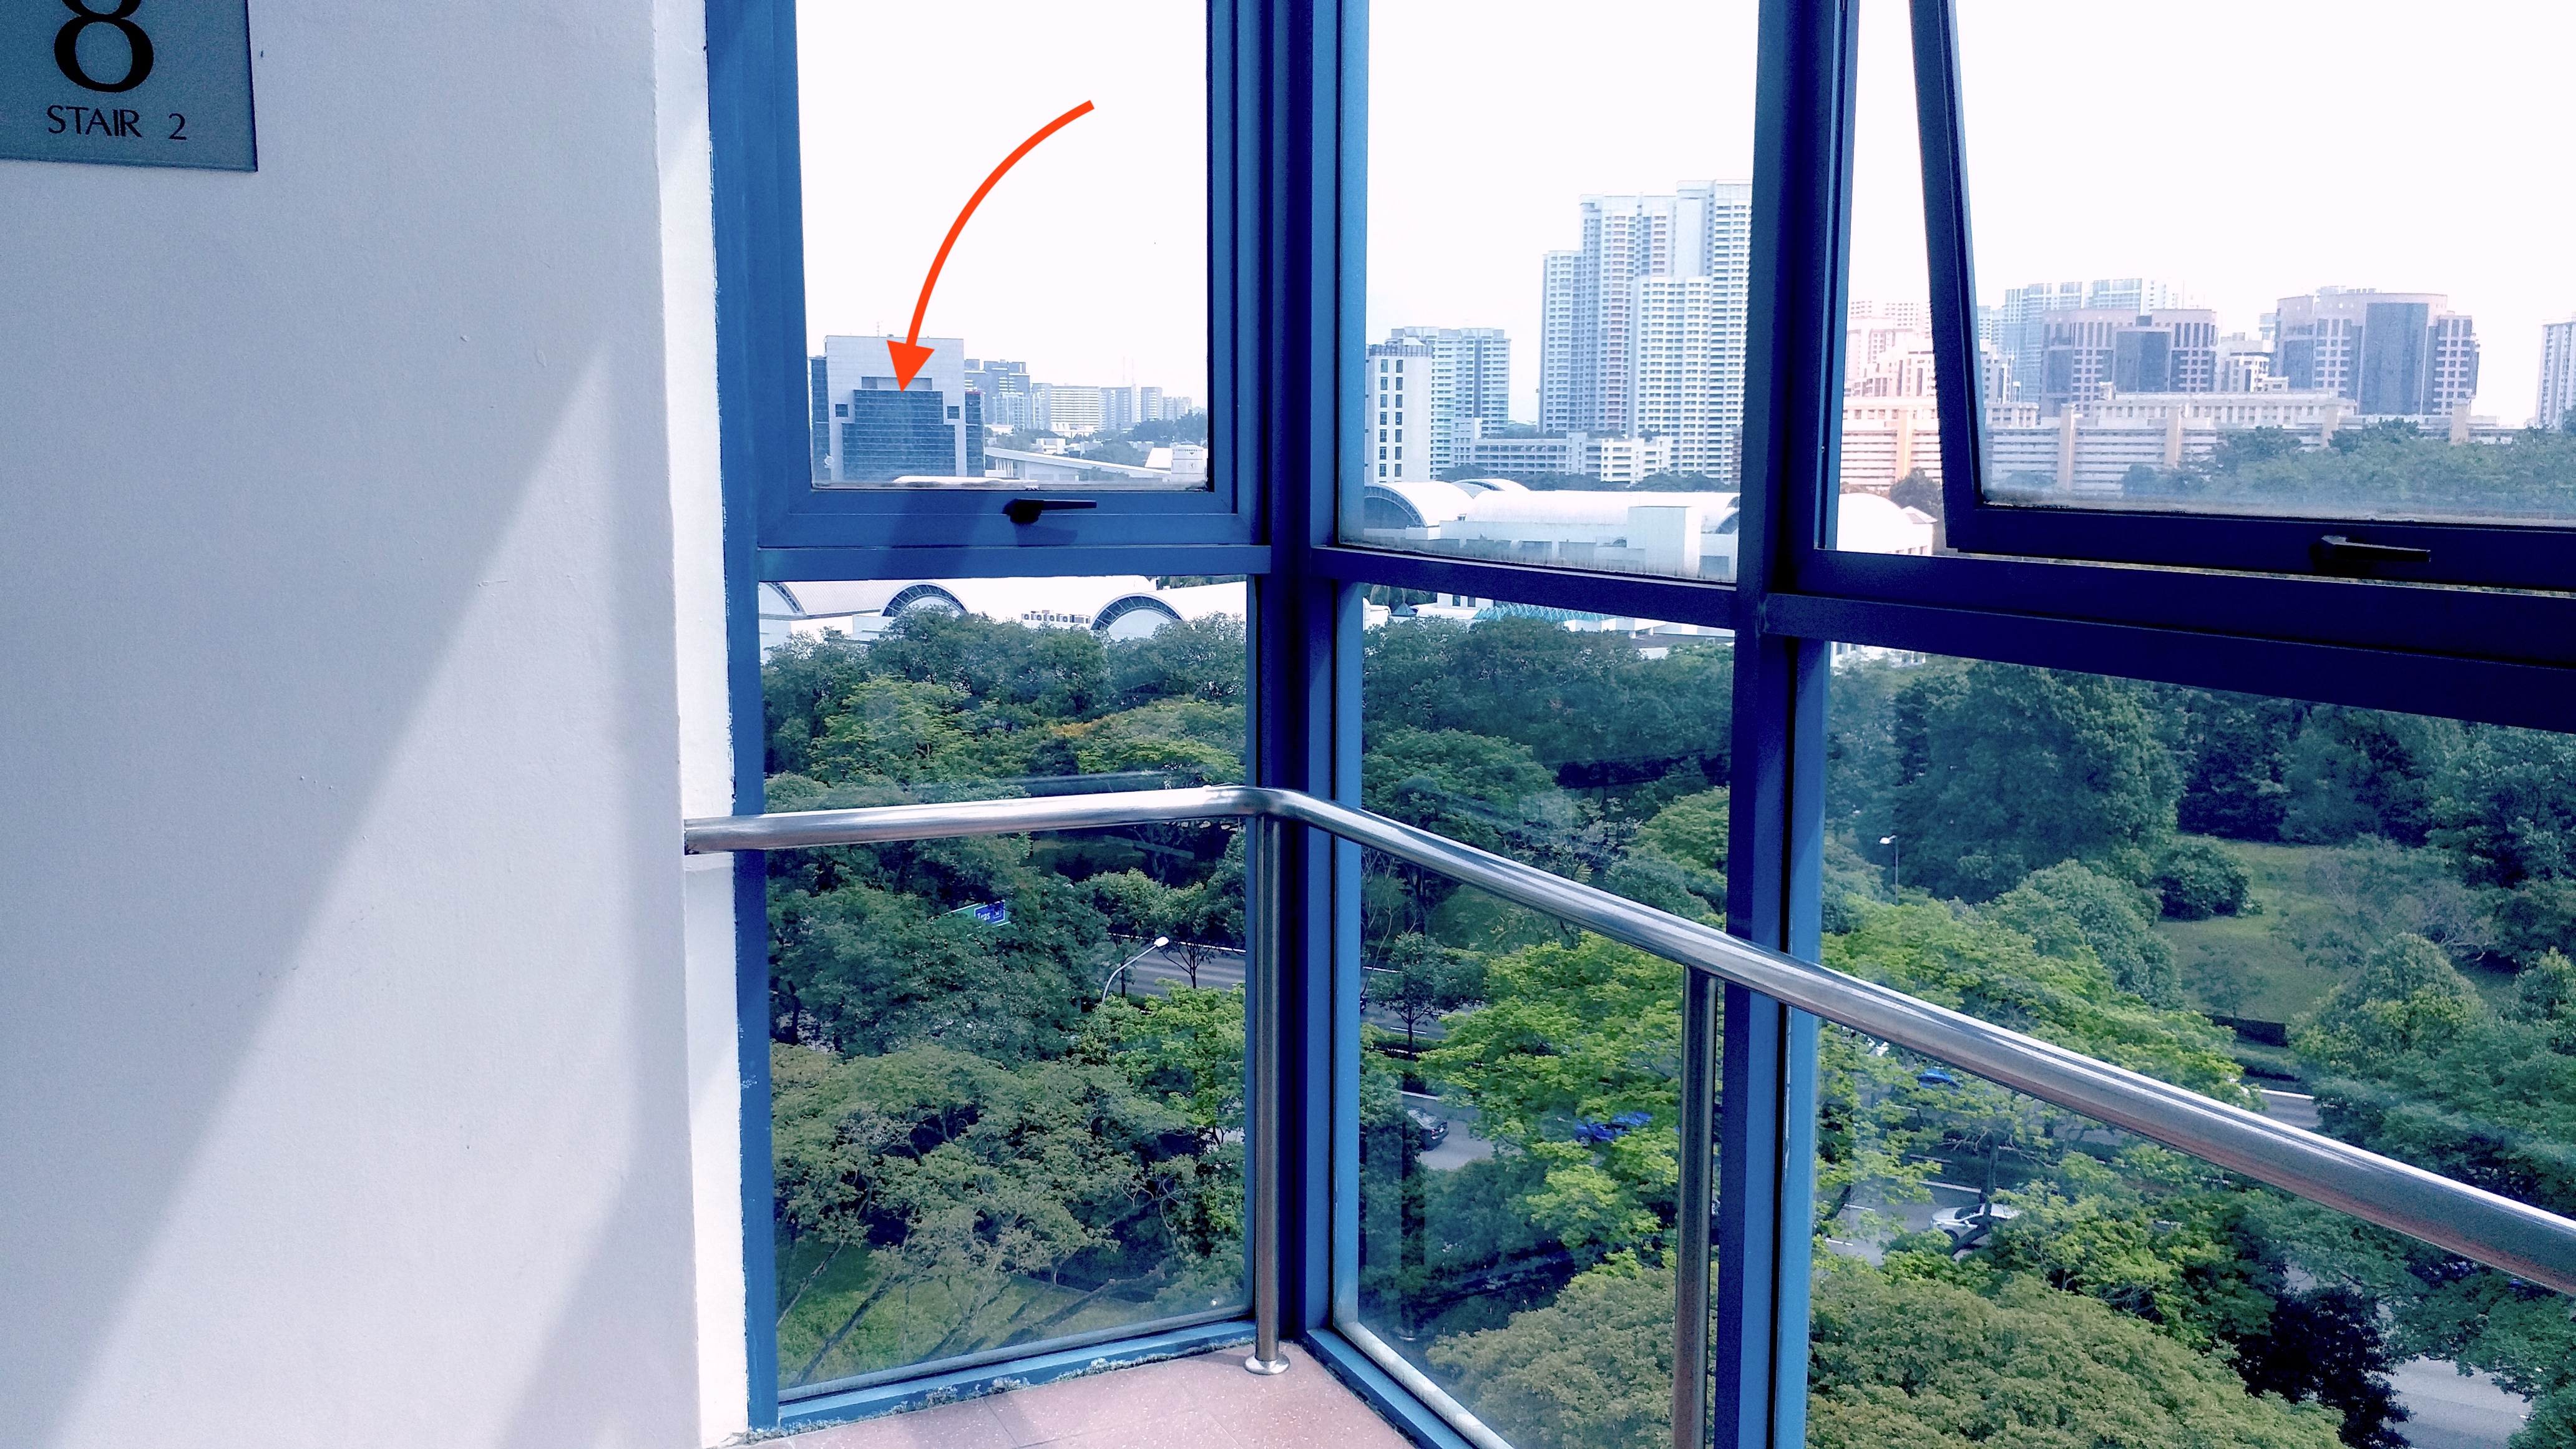
\includegraphics[width=0.5\textwidth]{figures/context.jpg}
		\caption{A Raspberry Pi-based camera was mounted on this window,}
		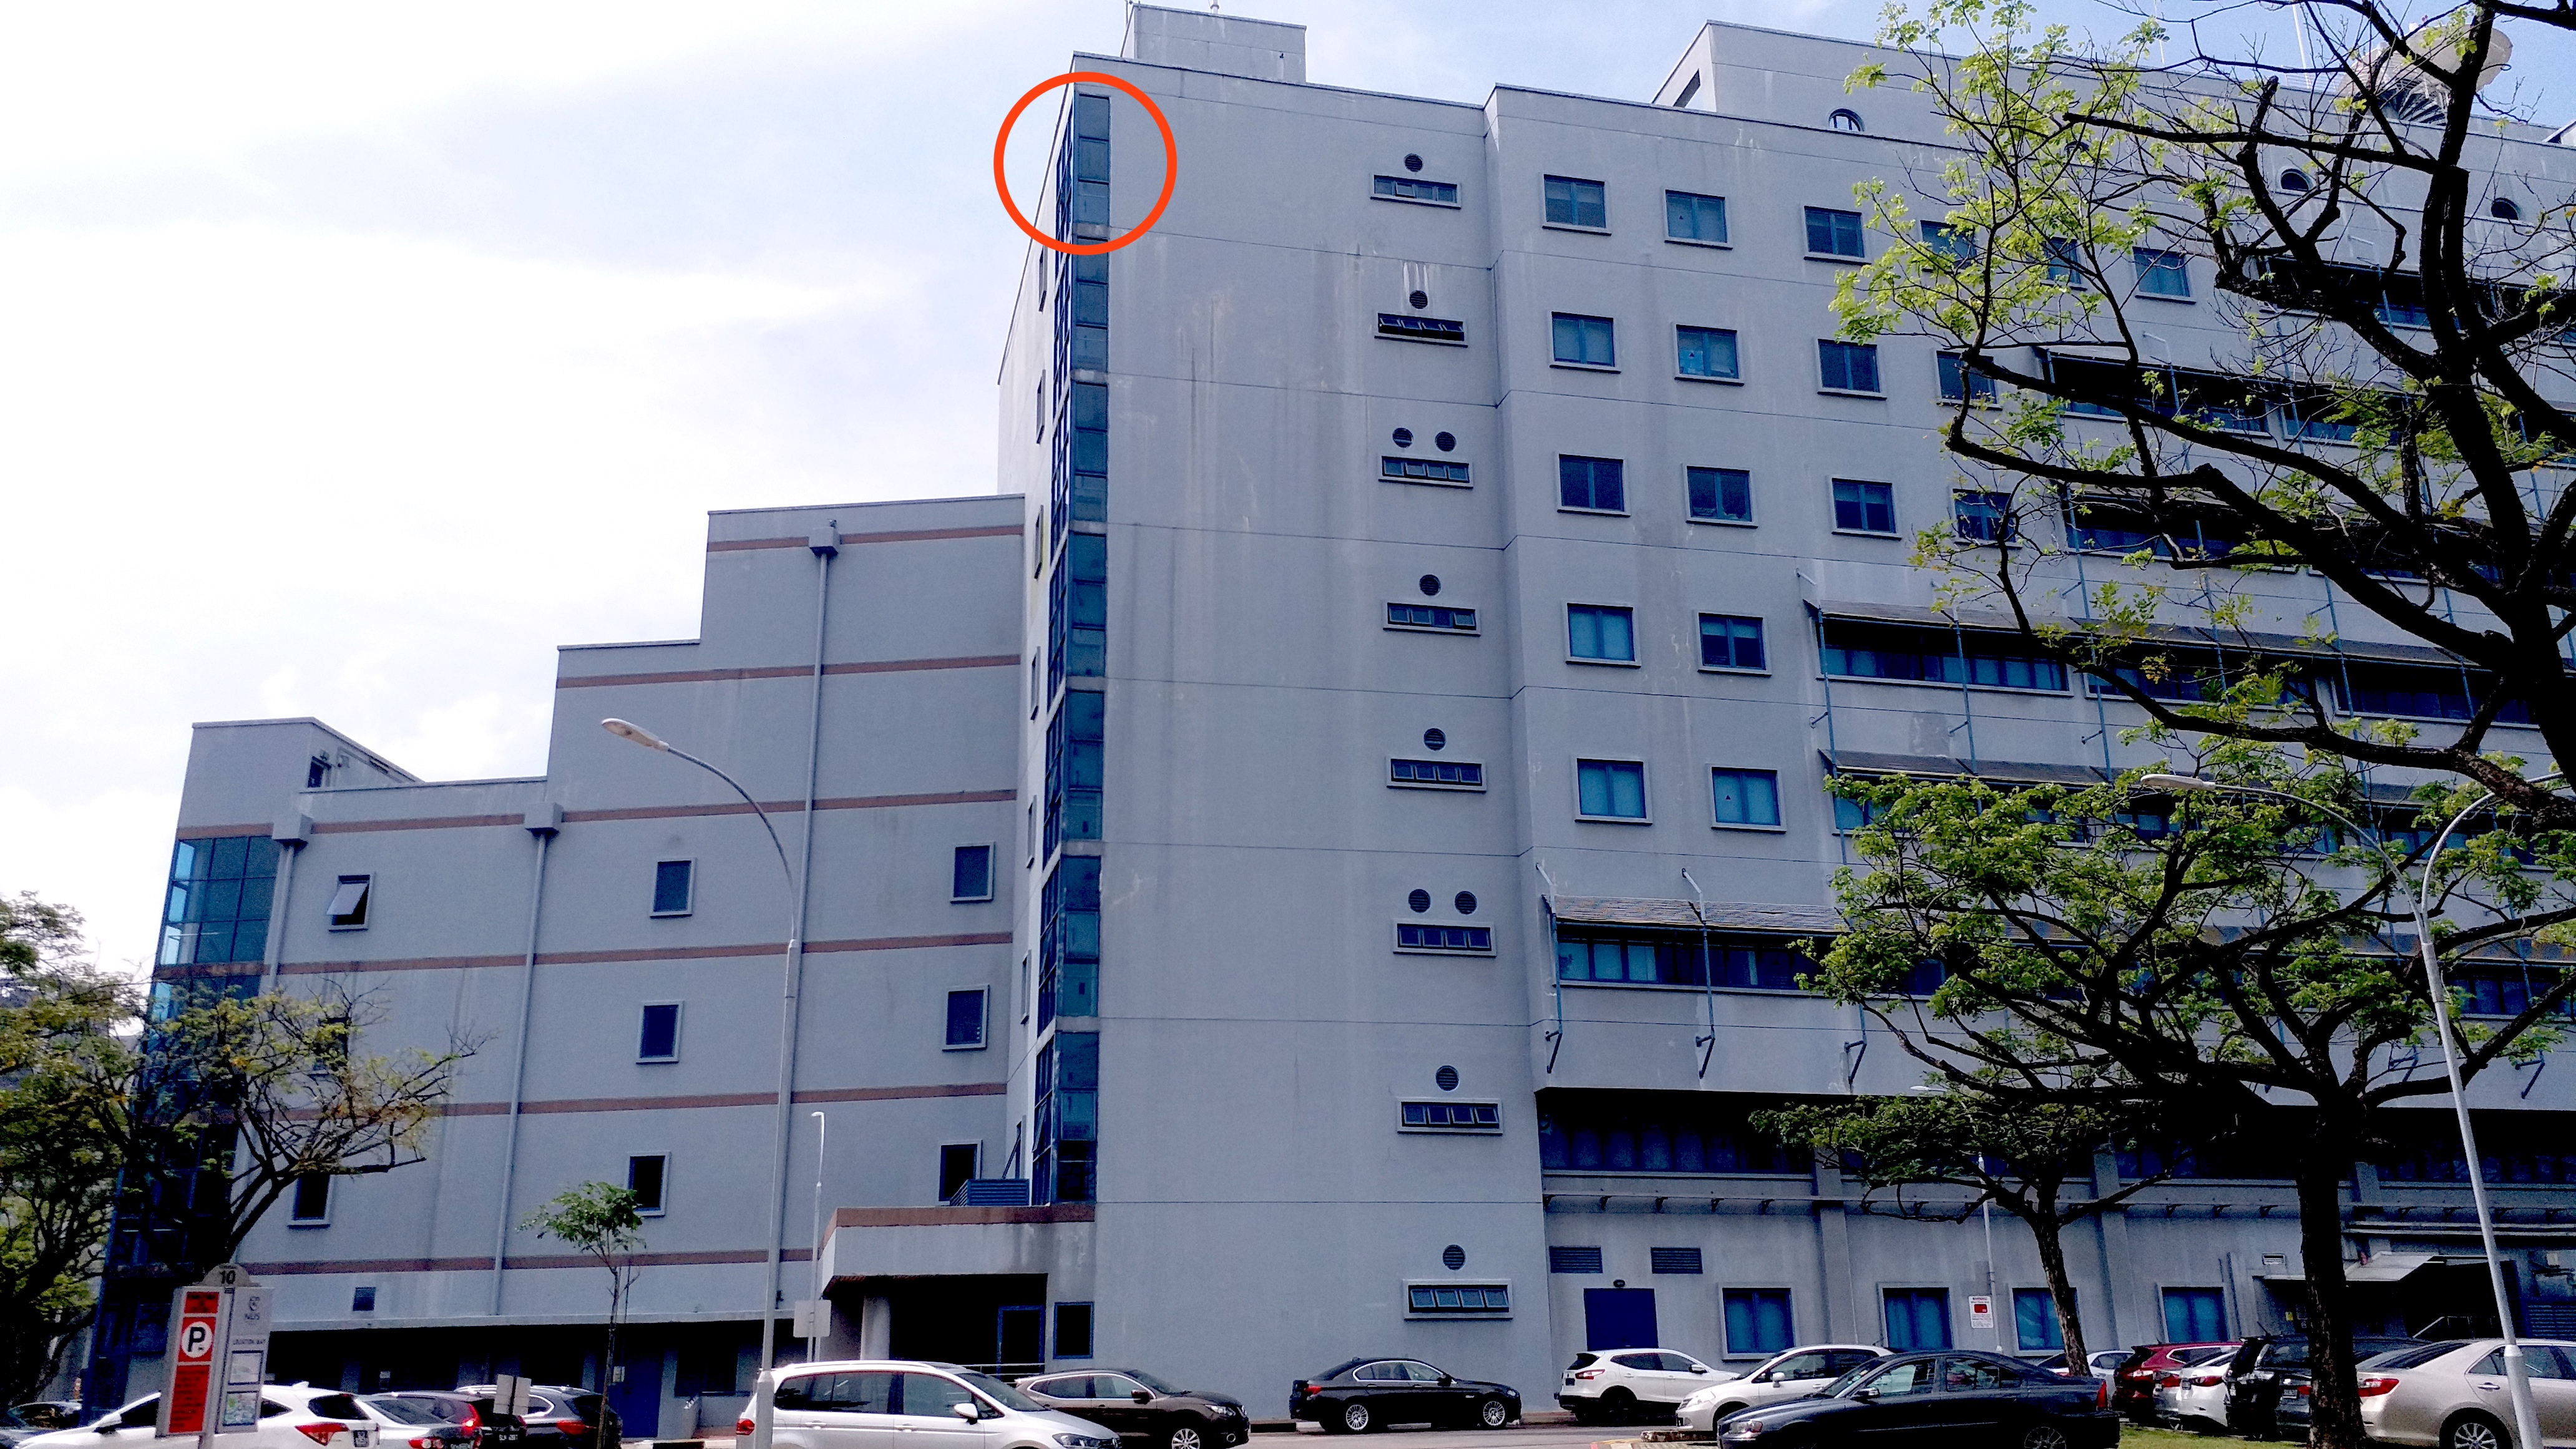
\includegraphics[width=0.5\textwidth]{figures/context_2.jpg}
		\caption{located at the encircled position,}
		\vskip 5mm
		\includegraphics[width=0.5\textwidth]{figures/spots_wo_labels.png}
		\caption{facing the following parking lot.}
	\end{figure}
	\begin{figure}[H]
		\centering
		\includegraphics[width=0.8\textwidth]{figures/spots_w_labels.png}
		\caption{Each spot was assigned an ID for cropping and file-naming purposes.}
	\end{figure}

\begin{enumerate}
	\item Construction of an Arduino-based camera to take pictures of an NUS parking lot over the 
	course of about thirty days, in the manner of \textit{PKLot}. Then, to clean, label, securely store, 
	and use this data to create CNNs.
	\begin{adjustwidth}{6mm}{}
		Doing so will help us understand the practical challenges involved in the collection of  
		data appropriate for our use: such challenges could pertain to security, infrastructure, 
		environment,  etc.
	\end{adjustwidth}
\end{enumerate}
\newpage
The first objective is to be addressed soon: an Arduino-based camera is being prepared and will 
likely be gathering data through the month of May. This device will comprise of the following parts:
\begin{enumerate}
	\item Arduino Uno (an inexpensive microcontroller).
	\item A five-megapixel camera module.
	\item 64 GB microSD card.
	\item Rechargeable 5200 mAh battery (with a protective sleeve).
\end{enumerate}

We have taken inspiration from \textit{PKLot} in the creation of the data collection schedule: a 
picture of the selected parking lot will be taken every five minutes during working hours over the 
course of thirty days. This will total to about 2,880 pictures. Given that there are about 50 spots 
in the selected lot, we will have about 140,000 examples to train and test our CNN on, after images
of 	individual spots have been extracted from the pictures in the manner of figures 14, 15, and 16. 
We intend to gather such a large number of examples because many issues that prevent neural 
networks from training well are related to a lack of training examples.

Our selected parking lot is that  Pictures will be 
taken from a sufficiently-high vantage such that images cannot be used to identify people and car 
plates. Moreover, as soon as pictures are taken, they will be encrypted using 256-bit AES 
(Advanced Encryption Standard). This encryption helps protect the data against malicious 
individuals who attempt to steal the device. Moreover, the device will be regularly visited: given 
estimates of energy consumption, batteries will have to be replaced about every five days. After 
the data collection has finished, pictures will be deleted from the microSD card and transferred to 
FloydHub, where files can be accessed only by uploaders. FloydHub also uses 256-bit AES to 
communicate with local machines to run jobs. They have taken measures to restrict the number of 
users (to just two) who have administrative access to their servers. Finally, user passwords and 
authentication tokens are not managed by them, but by Auth0. We believe this is more than 
sufficient for our application and data.

\hspace*{-6mm}The following is visual context to our data collection:

\newpage
The approach to the second objective, creation of the mobile application, is dependent on the 
experiences from the first. Namely, the second objective will require upgrade of the camera to one 
that is Internet-connected; powering and reliably connecting such a device can be challenging. 
Moreover, the CNN will need to be placed on the cloud, with a suitable interface to handle 
communication between the camera(s) taking the picture upon user request, the model serving 
the prediction, and the user's mobile application. Amazon's Amazon Web Services offers us tools 
to host CNNs on the cloud~\cite{aws}\relax. They offer serverless services that can scale 
dynamically in capacity in response to demand, and are only billed per user request. Our 
application intends to harness such services in its back-end.

\section{Conclusion and extensions}
The use of CNNs to ascertain the occupancy of parking lots has shown good promise, and is soon 
to be applied to the local context. Nonetheless, increasing the resolution of information available to 
those seeking a parking spot is not the only implication of this project, especially given that NUS' 
parking lots are organized appropriately for demand. Rather, we truly view this project as a 
capability-building exercise; a segue into greater problems that can be addressed by machine 
learning--either by us or those who take reference to our experiences in the future.

\newpage
\begin{thebibliography}{unsrt}
    \bibitem{pklot-paper}
		Almeida, P. R., Oliveira, L. S., Britto, A. S., Silva, E. J., \& Koerich, A. L. (2015). PKLot--A robust 
		dataset for parking lot classification. \textit{Expert Systems with Applications}, 42(11), 
		4937-4949. doi:10.1016/j.eswa.2015.02.009
\end{thebibliography}

\end{document}